\pdfoutput=1
\documentclass[red,handout,professionalfont]{beamer}
% \documentclass[red,professionalfont]{beamer}
\usepackage{multimedia}
\usepackage{url}
\usepackage{amssymb}  % the check symbol 
% Python listing setup

\usepackage{color}
\usepackage[procnames]{listings}
\usepackage{textcomp}
\usepackage{setspace}
\usepackage{palatino}
\renewcommand{\lstlistlistingname}{Code Listings}
\renewcommand{\lstlistingname}{Code Listing}
\definecolor{gray}{gray}{0.5}
\definecolor{green}{rgb}{0,0.5,0}
\definecolor{lightgreen}{rgb}{0,0.7,0}
\definecolor{purple}{rgb}{0.5,0,0.5}
\definecolor{darkred}{rgb}{0.5,0,0}
\lstnewenvironment{python}[1][]{
\lstset{
language=python,
breaklines=true,
basicstyle=\ttfamily\small\setstretch{1},
stringstyle=\color{green},
showstringspaces=false,
alsoletter={1234567890},
otherkeywords={\ , \}, \{},
keywordstyle=\color{blue},
emph={access,and,as,break,class,continue,def,del,elif,else,%
except,exec,finally,for,from,global,if,import,in,is,%
lambda,not,or,pass,print,raise,return,try,while,assert},
emphstyle=\color{orange}\bfseries,
emph={[2]self},
emphstyle=[2]\color{gray},
emph={[4]ArithmeticError,AssertionError,AttributeError,BaseException,%
DeprecationWarning,EOFError,Ellipsis,EnvironmentError,Exception,%
False,FloatingPointError,FutureWarning,GeneratorExit,IOError,%
ImportError,ImportWarning,IndentationError,IndexError,KeyError,%
KeyboardInterrupt,LookupError,MemoryError,NameError,None,%
NotImplemented,NotImplementedError,OSError,OverflowError,%
PendingDeprecationWarning,ReferenceError,RuntimeError,RuntimeWarning,%
StandardError,StopIteration,SyntaxError,SyntaxWarning,SystemError,%
SystemExit,TabError,True,TypeError,UnboundLocalError,UnicodeDecodeError,%
UnicodeEncodeError,UnicodeError,UnicodeTranslateError,UnicodeWarning,%
UserWarning,ValueError,Warning,ZeroDivisionError,abs,all,any,apply,%
basestring,bool,buffer,callable,chr,classmethod,cmp,coerce,compile,%
complex,copyright,credits,delattr,dict,dir,divmod,enumerate,eval,%
execfile,exit,file,filter,float,frozenset,getattr,globals,hasattr,%
hash,help,hex,id,input,int,intern,isinstance,issubclass,iter,len,%
license,list,locals,long,map,max,min,object,oct,open,ord,pow,property,%
quit,range,raw_input,reduce,reload,repr,reversed,round,set,setattr,%
slice,sorted,staticmethod,str,sum,super,tuple,type,unichr,unicode,%
vars,xrange,zip},
emphstyle=[4]\color{purple}\bfseries,
upquote=true,
morecomment=[s][\color{lightgreen}]{"""}{"""},
commentstyle=\color{red}\slshape,
literate={>>>}{\textbf{\textcolor{darkred}{>{>}>}}}3%
         {...}{{\textcolor{gray}{...}}}3,
procnamekeys={def,class},
procnamestyle=\color{blue}\textbf,
framexleftmargin=1mm, framextopmargin=1mm,% frame=shadowbox,
%rulesepcolor=\color{blue},
#1
}}{}


\usepackage{tikz}
\usetikzlibrary{decorations.pathreplacing}
%\bibliography{mujstyl}
\theoremstyle{definition}
\newtheorem{definice}{Definition}[section]
\newtheorem{thm}{Theorem}[section]
\newtheorem{idea}{Idea}[section]
\newtheorem{cor}[thm]{Corrollary}
\newtheorem{lem}[thm]{Lemma}
\newtheorem{obs}[thm]{Observation}
\newtheorem{rem}[thm]{Remark}
\newtheorem{ex}[thm]{Example}
\newtheorem{quizz}[thm]{Question}
\newcommand{\pomega}{\mbox{$\mathcal{P}(\omega)$}}
\newcommand{\cont}{\mbox{$\mathfrak c$}}
\newcommand{\ba}{\mbox{${\mathbb B}$}}
\newcommand{\0}{\mbox{${\bf 0}$}}
\newcommand{\F}{\mbox{${\mathcal F}$}}
\newcommand{\rest}{\mbox{$\upharpoonright$}}
\newcommand{\cl}[1]{\mbox{$\overline{#1}$}}
\newcommand{\yes}{\textcolor{green}{$\checkmark$}}
\newcommand{\no}{\textcolor{red}{$\times$}}
\renewcommand{\emph}[1]{{\bf #1}}
\mode<presentation>
{
\useinnertheme{rounded}

\usecolortheme{whale}
\usecolortheme{orchid}

\setbeamerfont{block title}{size={}}

%   \useoutertheme{default}
%   \usetheme{Copenhagen}
%   \useoutertheme{default}
  \setbeamercovered{invisible}
}
\setbeamertemplate{navigation symbols}{} 
\usepackage[utf8]{inputenc}
\usepackage[czech,english]{babel}
\usepackage{lmodern}
%\usepackage{times}
\usepackage[T1]{fontenc}


\title[]{Rychlokurz Pythonu}
% \author[]{Jonathan L. Verner}
% \institute[Charles University, Prague] % (optional,but mostly needed)
% {
%   Department of Logic\\
%   Faculty of Philosophy\\
%   Charles University in Prague
% }
\date[]{}
% \subject{}
%\pgfdeclareimage[height=1cm]{university-logo}{UK-logo}
%\logo{\pgfuseimage{university-logo}}

\begin{document}

\AtBeginSection[]
{
  \begin{frame}<beamer>
    \begin{block}{}
%    \begin{centering}
    \hfill\insertsection\hfill\
 %   \end{centering}
    \end{block}
    %\tableofcontents[currentsection]
  \end{frame}
}

\AtBeginSubsection[]
{
  \begin{frame}<beamer>
    \begin{block}{}
  %  \begin{centering}
    \hfill\insertsubsection\hfill\
   % \begin{centering}
    \end{block}
    %\tableofcontents[currentsection]
  \end{frame}
}

%#################################################################

\begin{frame}{} \titlepage
%{\ \hfill \includegraphics[width=1cm]{UK-logo}\hfill\ }
\end{frame}

\begin{frame}\frametitle{Naučte se Python za 10 minut}
 \begin{center}
  
\includegraphics[width=3cm]{python_logo.png}
  
  \url{python.org}\pause
  
  \url{wiki.python.org/moin/BeginnersGuide/Programmers}\pause
  
  \url{www.acm.uiuc.edu/sigunix/workshops/crashpython/crashpython.pdf}
 \end{center}
\end{frame}

\begin{frame}\frametitle{Instalace, spouštění}
 \begin{block}{}
\ \hfill \url{www.python.org}\hfill\
\end{block}
\begin{itemize}
 \item Sekce download
 \item verze \emph{2.něco} (2.7)
\end{itemize}
\begin{center}
\url{http://python.org/ftp/python/2.7.2/python-2.7.2.msi}
\end{center}\pause
\begin{itemize}
 \item program IDLE --- integrované vývojové prostředí \pause
\end{itemize}
\begin{center}
\begin{minipage}{4cm}
 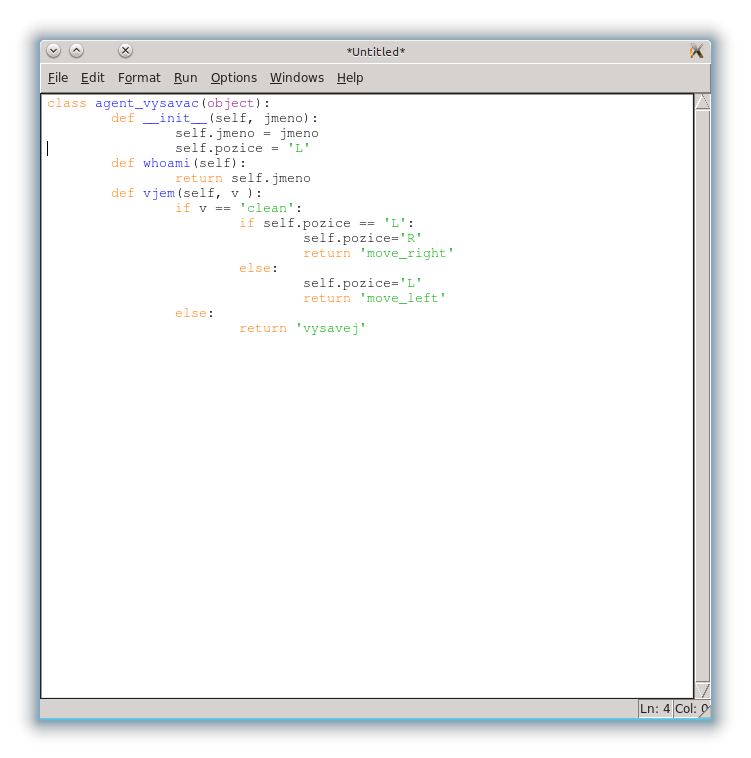
\includegraphics[height=4cm]{idle-screenshot-editor.png}
\end{minipage}
\begin{minipage}{4cm}
 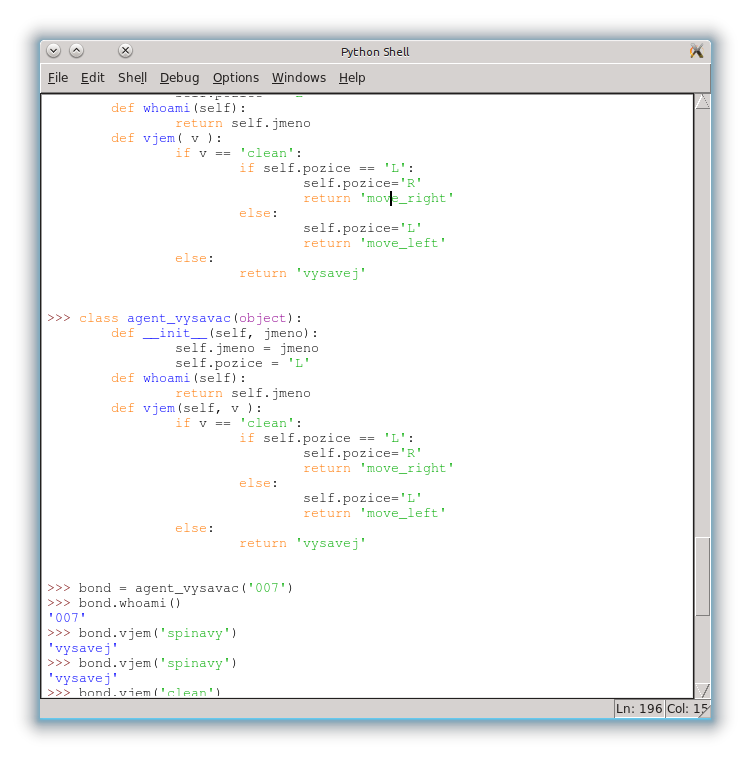
\includegraphics[height=4cm]{idle-screenshot-interpreter.png}
\end{minipage}
\end{center}
\end{frame}

\begin{frame}[fragile]\frametitle{Datové typy}
 \begin{itemize}
  \item čísla\pause
  \item řetězce\pause
  \item seznamy\pause
  \item tice\pause
  \item slovníky\pause
  \item moduly\pause
  \item objekty
 \end{itemize}
\end{frame}


\begin{frame}[fragile]\frametitle{Čísla}
 \begin{itemize}
  \item celá čísla
  \begin{python}
>>> a=3
>>> a/2
1
>>> a%2
1
>>> c=25**25
>>> print c
88817841970012523233890533447265625
  \end{python}
  \item \uv{floating point}
  \begin{python}
>>> a=3.0
>>> a/2
1.5
>>> c=25.0**25.0
>>> print c
8.881784197e+34   
  \end{python}
\end{itemize}
\end{frame}

\begin{frame}[fragile]\frametitle{Řetězce}
  \begin{python}
>>> s = "Ahoj"
>>> s.upper()
'AHOJ'
>>> s = s + " svete!"
>>> print s
Ahoj svete!
>>> print s[1:4]
hoj
>>> len(s)
11
>>> s.index('sv')
5
>>> s = s+str(78)
>>> print s
Ahoj svete!78
  \end{python}
\end{frame}

\begin{frame}[fragile]\frametitle{Seznamy}
\begin{minipage}{4.9cm}
\begin{python}
>>> l = [1,7,2,'Hi',9]
>>> l.sort()
>>> l
[1, 2, 7, 9, 'Hi']
>>> l[2:]
[7, 9, 'Hi']
>>> del l[1]
>>> l
[1, 7, 9, 'Hi']
>>> l[-1]
'Hi'
>>> l = l + l
>>> l
[1, 7, 9, 'Hi', 1, 7, 9, 'Hi']
\end{python}\pause
\end{minipage}
\begin{minipage}{5.7cm}
{\small
 \begin{itemize}
  \item[] {\bf append(x)} přidá {\tt x} na konec
  \item[] {\bf extend(L)} prodlouží o seznam {\tt L}
  \item[] {\bf insert(i,x)} vloží {\tt x} na {\tt i}-tou pozici
  \item[] {\bf remove(x)} odstraní první {\tt x}
  \item[] {\bf pop()} odstraní poslední prvek a vrátí ho
  \item[] {\bf index(x)} vrátí pozici prvního {\tt x}
  \item[] {\bf count(x)} vrátí počet výskytů {\tt x}
  \item[] {\bf sort()} uspořádá seznam
  \item[] {\bf reverse()} obrátí seznam
 \end{itemize}
 }
\end{minipage}


\end{frame}

\begin{frame}[fragile]\frametitle{Slovníky}
\begin{minipage}{6.3cm}
  \begin{python}
>>> s='cislo'
>>> d = { 'spd':25, 'col':"red", 1:s }
>>> d['spd']
25
>>> len(d)
3
>>> 'col' in d
True
>>> d[2/2]
'cislo'
>>> del d[1]
>>> d
{'spd': 25, 'col': 'red'}    
  \end{python} 
\end{minipage}
\begin{minipage}{4cm}
{\small
\begin{itemize}
 \item[] {\bf items()} vrátí seznam dvojic (klíč, hodnota)
 \item[] {\bf keys()} vrátí seznam klíčů
 \item[] {\bf values()} vrátí seznam hodnot
\end{itemize}
}
\end{minipage}
\end{frame}

\begin{frame}[fragile]\frametitle{If, for, while}
\begin{minipage}{7cm}
\begin{python}
while n > 0:
  if True and n%2 == 0:
    print n,
  elif n == 9:
    for s in [ 'a','b','c']:
      print s
      if s == 'b':
        break
      elif s == 'c':
        pass
  n = n - 1
\end{python}\pause
\end{minipage}
\begin{minipage}{3cm}
\begin{python}
10 a
b
8 6 4 2
\end{python}\pause
\end{minipage}

\begin{itemize}
 \item odsazení se používá místo závorek (C, C++, Java), {\tt begin}, {\tt end} (Pascal)\pause
 \item kladná čísla, {\tt True}, neprázdné seznamy se vyhodnocují jako true\pause
 \item 0, {\tt False}, prázdné seznamy, {\tt None} se vyhodnocují jako false
\end{itemize}

\end{frame}

\begin{frame}[fragile]\frametitle{Funkce}
\begin{python}
def ahoj(jmeno):
  print "Ahoj", jmeno, "!"

def fact(a):
  """ Spocte faktorial cisla a """
  if a > 1:
    return a*fact(a-1)
  return 1
\end{python}\pause
\begin{python}
>>> fact(10)
3628800
>>> ahoj("Vileme")
Ahoj Vileme !
\end{python}
\end{frame}
\begin{frame}[fragile]\frametitle{Třídy}
\begin{python}
class agent_vysavac(object):
  """Jednoduchy agent vysavac, ktery se pohybuje na dvou polich L (levem) a P (pravem) a vysava """
  
  def __init__(self, jmeno):
    """Toto je konstruktor, zavola se vzdy pri vytvoreni agenta"""
    self.jmeno = jmeno
    self.pozice = 'L'
  
  def whoami(self):
    return self.jmeno
\end{python}
\end{frame}

\begin{frame}[fragile]\frametitle{Třídy (pokračování)}
\begin{python}
  def vjem(self, v ):
    if v == 'clean':
      if self.pozice == 'L':
        self.pozice='R'
        return 'move_right'
      elif self.pozice == 'R':
        self.pozice='L'
        return 'move_left'
      else:
        self.explode()
    else:
      return 'vysavej'

  def explode(self):
    print "Agent " + self.jmeno + " explodoval"
\end{python}
\end{frame}

\begin{frame}[fragile]\frametitle{Agent vysavač}
\begin{python}
>>> bond = agent_vysavac('007')
>>> bond.whoami()
'007'
>>> bond.vjem('spinavy')
'vysavej'
>>> bond.vjem('spinavy')
'vysavej'
>>> bond.vjem('clean')
'move_right'
>>> bond.vjem('clean')
'move_left'
>>> bond.vjem('clean')
'move_right'
>>> bond.vjem('spinavy')
'vysavej'
\end{python}
\end{frame}


% \begin{frame}[fragile]\frametitle{Datové typy II.}
% \begin{itemize}
%   \item seznamy
%   \begin{python}
%    sz = [ 1, 2, 0.5, "Test", [1,2] ]
%   \end{python}
%   \item n-tice
%   \begin{python}
%     d = (1,2)
%     d = (1.5,2.5,3.5)
%     d = (sz,a)
%   \end{python}
%   \item slovníky
%   \begin{python}
%     d = { 'speed':25, 'barva':"modra", 1:s }
%     d["speed"] = 37
%     print d['barva']
%   \end{python}
% 
%   \item objekty
%   \item moduly
%  \end{itemize}
% 
% \end{frame}



\end{document}
